\documentclass[pra,
superscriptaddress,
amssymb,amsmath,amsmath,showpacs,reprint,twocolumn]{revtex4-1}
\usepackage{color}
\usepackage{graphicx}
\usepackage{epstopdf}
\usepackage{natbib}
\usepackage{wasysym}
\usepackage{hyperref}
\usepackage{dcolumn}

\hypersetup{%
   pdfpagemode=None, %FullScreen,
   pdfstartpage=1,
   pdfstartview=FitH,
   pdfmenubar=true,
   pdftoolbar=true,
   colorlinks = true,
   linkcolor=blue,
   citecolor=blue,
   bookmarksopen=false
}


\def\half{\frac{1}{2}}

\usepackage{booktabs}
\usepackage{multirow}
\usepackage{graphicx}
\usepackage{amsmath}
\usepackage{indentfirst}
\pagenumbering{arabic}

\usepackage[utf8]{inputenc}
\usepackage[T1]{fontenc}
\usepackage{fontspec}
\usepackage[polish]{babel}
\usepackage{amsmath}
\usepackage{graphicx}
\usepackage[table,xcdraw]{xcolor}
\usepackage{hhline}
\usepackage{placeins}
\usepackage[margin=0.6in]{geometry}
\usepackage{appendix}
\usepackage{float}
\usepackage{caption}
\usepackage{subcaption}
\usepackage{colortbl}
\usepackage{physics}
\usepackage{datetime}
\usepackage[shortlabels]{enumitem}
\usepackage{diagbox}
\usepackage{booktabs}
\usepackage{multirow}
\usepackage{indentfirst}
\usepackage{tikz}
\usetikzlibrary{calc}


% \date{\today}
% \setlength\parindent{0pt}

\newcommand{\com}[1]{{\color{red} #1}}

\newcommand{\link}[2]{{\color{cyan} \href{#1}{#2}}}

\renewcommand{\emph}{\textbf}

\DeclareDocumentCommand{\hcancel}{mO{0pt}O{0pt}O{0pt}O{0pt}}{%
    \tikz[baseline=(tocancel.base)]{
        \node[inner sep=0pt,outer sep=0pt] (tocancel) {#1};
        \draw[red] ($(tocancel.south west)+(#2,#3)$) -- ($(tocancel.north east)+(#4,#5)$);
    }%
}%

\begin{document}
\title{Doświadczenie J14: Pomiar zasięgu, rozrzutu zasięgu i zdolności hamującej cząstek alfa w powietrzu}
\author{\sc Kacper Cybiński}
\email{e-mail: k.cybinski@student.uw.edu.pl}
\affiliation{\sl Faculty of Physics, University of Warsaw, Pasteura 5, 02-093 Warsaw, Poland}
\date{\today}



\begin{abstract}
    Przedmiotem doświadczenia były pomiary zachowania cząstek alfa w powietrzu: zasięgu, rozrzutu zasięgu (straggling) i zdolności hamującej. W wyniku analizy danych uzyskano szukane zależności, oraz przedstawiono rozważania na temat uzyskanych wyników. Wyznaczono średni zasięg i rozrzut cząstek $\alpha$ w powietrzu jako odpowiednio $\bar{R} = 3.253 \pm 0.002$\,cm i $\sigma_r = (8.649 \pm 0.004)\cdot 10^{-2}$\,cm.
\end{abstract}

\maketitle

\section{Wstęp}

% Fizyka jądrowa, a w szczególności zachowania naładowanych cząstek o dawna fascynuje naukowców, którzy badają tę dziedzinę, oraz niezmiennie rozpala wyobraźnię i inspiruje kolejne młode pokolenia do zainteresowania nauką. Niestety jednak ze względu na mnogość niebezpieczeństw związanych z materiałami radioaktywnymi, możliwość zbadania próbki radioaktywnej nie jest czymś, co można zrobić w swoim garażu, tylko wymaga specjalistycznego sprzętu, który jest przeznaczony do badań naukowych. Po środku jednak między pełnoskalowymi doświadczeniami naukowymi a nauką w domowym zaciszu stoją kontrolowane eksperymenty mające na celu wprowadzanie w świat poważnej nauki, jak omawiany w tym tekście eksperyment z badaniem zachowania naładowanej cząstki alfa w powietrzu.

Omawiane w tym raporcie doświadczenie ma za zadanie wprowadzić studenta w tematykę badania zachowania naładowanych cząstek w materiałch, oraz pokazanie czego można się dowiedzieć o naturze cząstki, oraz świata w którym wchodzi w interakcję z obserwacji pomiarów. W tym przypadku badaną cząstką jest $\alpha$, wchodząca w interakcję z powietrzem. Z tego rodzaju interakcji można wyciągnąć w szczególności trzy interesujące nas wielkości, jakimi są zasięg cząstki w powietrzu, rozrzut zasięgu, oraz zdolność hamująca.   


\section{Wstęp Teoretyczny}

Ciężkie naładowane cząstki, do których zaliczamy cząstki $\alpha$ przechodząc przez ośrodek tracą energię głównie w wyniku zderzeń z elektronami ośrodka przez który podróżują, gdyż w wyniku tych zderzeń cząstki się jonizują i tracą małą porcję energii. Mimo, że strata w wyniku jednego zderzenia jest niewielka, to po złożeniu wielu zderzeń następujących po sobie sumaryczna strata energii może być znaczna. W szczególności po odpowiednio dużej ilości zderzeń cząstka może zostać w pełni zatrzymana, a odległość po jakiej to nastąpiło nazwiemy właśnie \emph{zasięgiem} $R$ cząstki.
Teoretycznie wydawać by się mogło, że podczas emisji takich samych cząstek o takiej samej energii ich zasięg powinien być taki sam, lecz ze względu na losową naturę zderzeń, które zabierają energię z cząstki, ten zasięg podlega pewnemu \emph{rozrzutowi} $\sigma_r$.
Jakkolwiek wielkość $R$ podlega pewnemu rozkładowi, to z dużo większą dokładnością jesteśmy w stanie określić odległość po jakiej wiązka cząstek jest osłabiana o połowę, więc to wydaje się być lepszym pomysłem na definicję zasięgu. Dla rozróżnienia oznaczmy go $\bar{R} $ i nazwiemy \emph{zasięgiem średnim}.
Ostatnia z wielkości, jakie bierzemy na warsztat to zdolność hamująca. Jest ona zdefiniowana jako strata energii na jednostkę długości: $S(E) = - \dd{E}/\dd{x}$ i w ogólnym przypadku jest dla ciężkich cząstek naładowanych opisywana wzorem Bethego-Blocha. Najbardziej ogólną jego postać można znaleźć w podręczniku A.Strzałkowskiego \cite{strzalkowski}, zaś w warunkach naszych cząstek $\alpha$, które lecą z prędkością nierelatywistyczną i po uproszczeniach wzór ten ma postać:
\begin{equation}\label{eq:bethe_bloch}
    -\dv{E}{x} = \kappa \frac{\rho z^2 m c^2}{2E} \frac{Z}{A} \log\frac{4 m_e c^2 E}{Imc^2}
\end{equation}
Gdzie $\kappa = 0.307$ MeV cm$^2$/g jest wielkością grupującą stałe z orginalnego wzoru, $\rho$ - gęstość ośrodka, $z$ - ładunek cząstki, $m$ - masa cząstki, $m_e$ - masa elektronu. Człon $\frac{Z}{A}$ przedstawia stosunek liczy masowej pierwiastka z którego składa się ośrodek, do liczby atomowej. Jako, że powietrze jest mieszanią przede wszystkim trzech gazów - Azotu, Tlenu i Argonu, to licząc ten ułamek wzięto wyniki dzielenia dla tych trzech pierwiastków, z wagami odpowiadającymi procentowej ich zawartości w powietrzu, tj odpowiednio $78.080\%$ N$_2$, $20.950\%$ O$_2$, $0.9340\%$ Ar.

Narysowawszy wykres straty energii w funkcji przebytej drogi widać, że straty energii rosną i osiągają maksimum dla końca toru lotu cząstki, a następnie szybko maleją w wyniku dominacji ekranowania ładunku cząstki przez wychwycone elektrony.

\section{Układ pomiarowy}

Układ pomiarowy wykorzystywany w tym doświadczeniu jest widoczny na Rys. \ref{fig:uklad}. Jest to zintegrowany układ firmy ORTEC, model Alpha Aria na który składa się szczelna komora testowa z zamontowaną w środku próbką $^{241}$Am, która emituje cząstki $\alpha$, odległego od próbki o $39.5$\,mm półprzewodnikowego detektora krzemowego, serii zaworów i pompy do manipulowania ciśnieniem powietrza w komorze, oraz ciśnieniomierza. Sygnał wychodzący z detektora był przekazywany do przedwzmacniacza, a następnie poprzez wzmacniacz liniowy i wielokanałowy analizator amplitudy kierowany do komputera, który zapisywał zliczenia cząstek na detektorze dla poszczególnych $4096$ kanałów. Dokładna zasada działania poszczególnych elementów jest opisana a Instrukcji do doświadczenia \cite{instrukcja}. Kanały analizatora odpowiadały różnym energiom padających cząstek $\alpha$, co podlegało kalibracji poprzez zmapowanie numerów kanałów do energii emitowanej przez źródło o dobrze znanej energii jakim był pulser o energii $5.276$\,MeV. 

Jak widać po opisie układu doświadczalnego, zamiast wyznaczania szukanych zachowań cząstki $\alpha$ dla różnych oddaleń próbki od detektora postanowiono emulować różne grubości warstwy powietrza poprzez modulację ciśnienia, tj ilości cząstek powietrza na objętość, przy stałej odległości. Jako, że odległość z ciśnieniem wiążą się linowo, to jest to bardzo naturalna zmiana w założeniach doświadczenia. Funkcję kalibracyjną tutaj dopasowywano na podstawie następujących trzech informacji: a) odległość do detektora w ciśnieniu atmosferycznym $1023$\,hPa wynosi $39.5$\,mm b) w czasie wykonywania pomiarów rzeczywiste ciśnienie atmosferyczne wynosiło $1004.9$\,hPa c) minimalne uzyskiwane ciśnienie w komorze to $0.004$\,mBa.

\begin{figure}[h!]
    \centering
    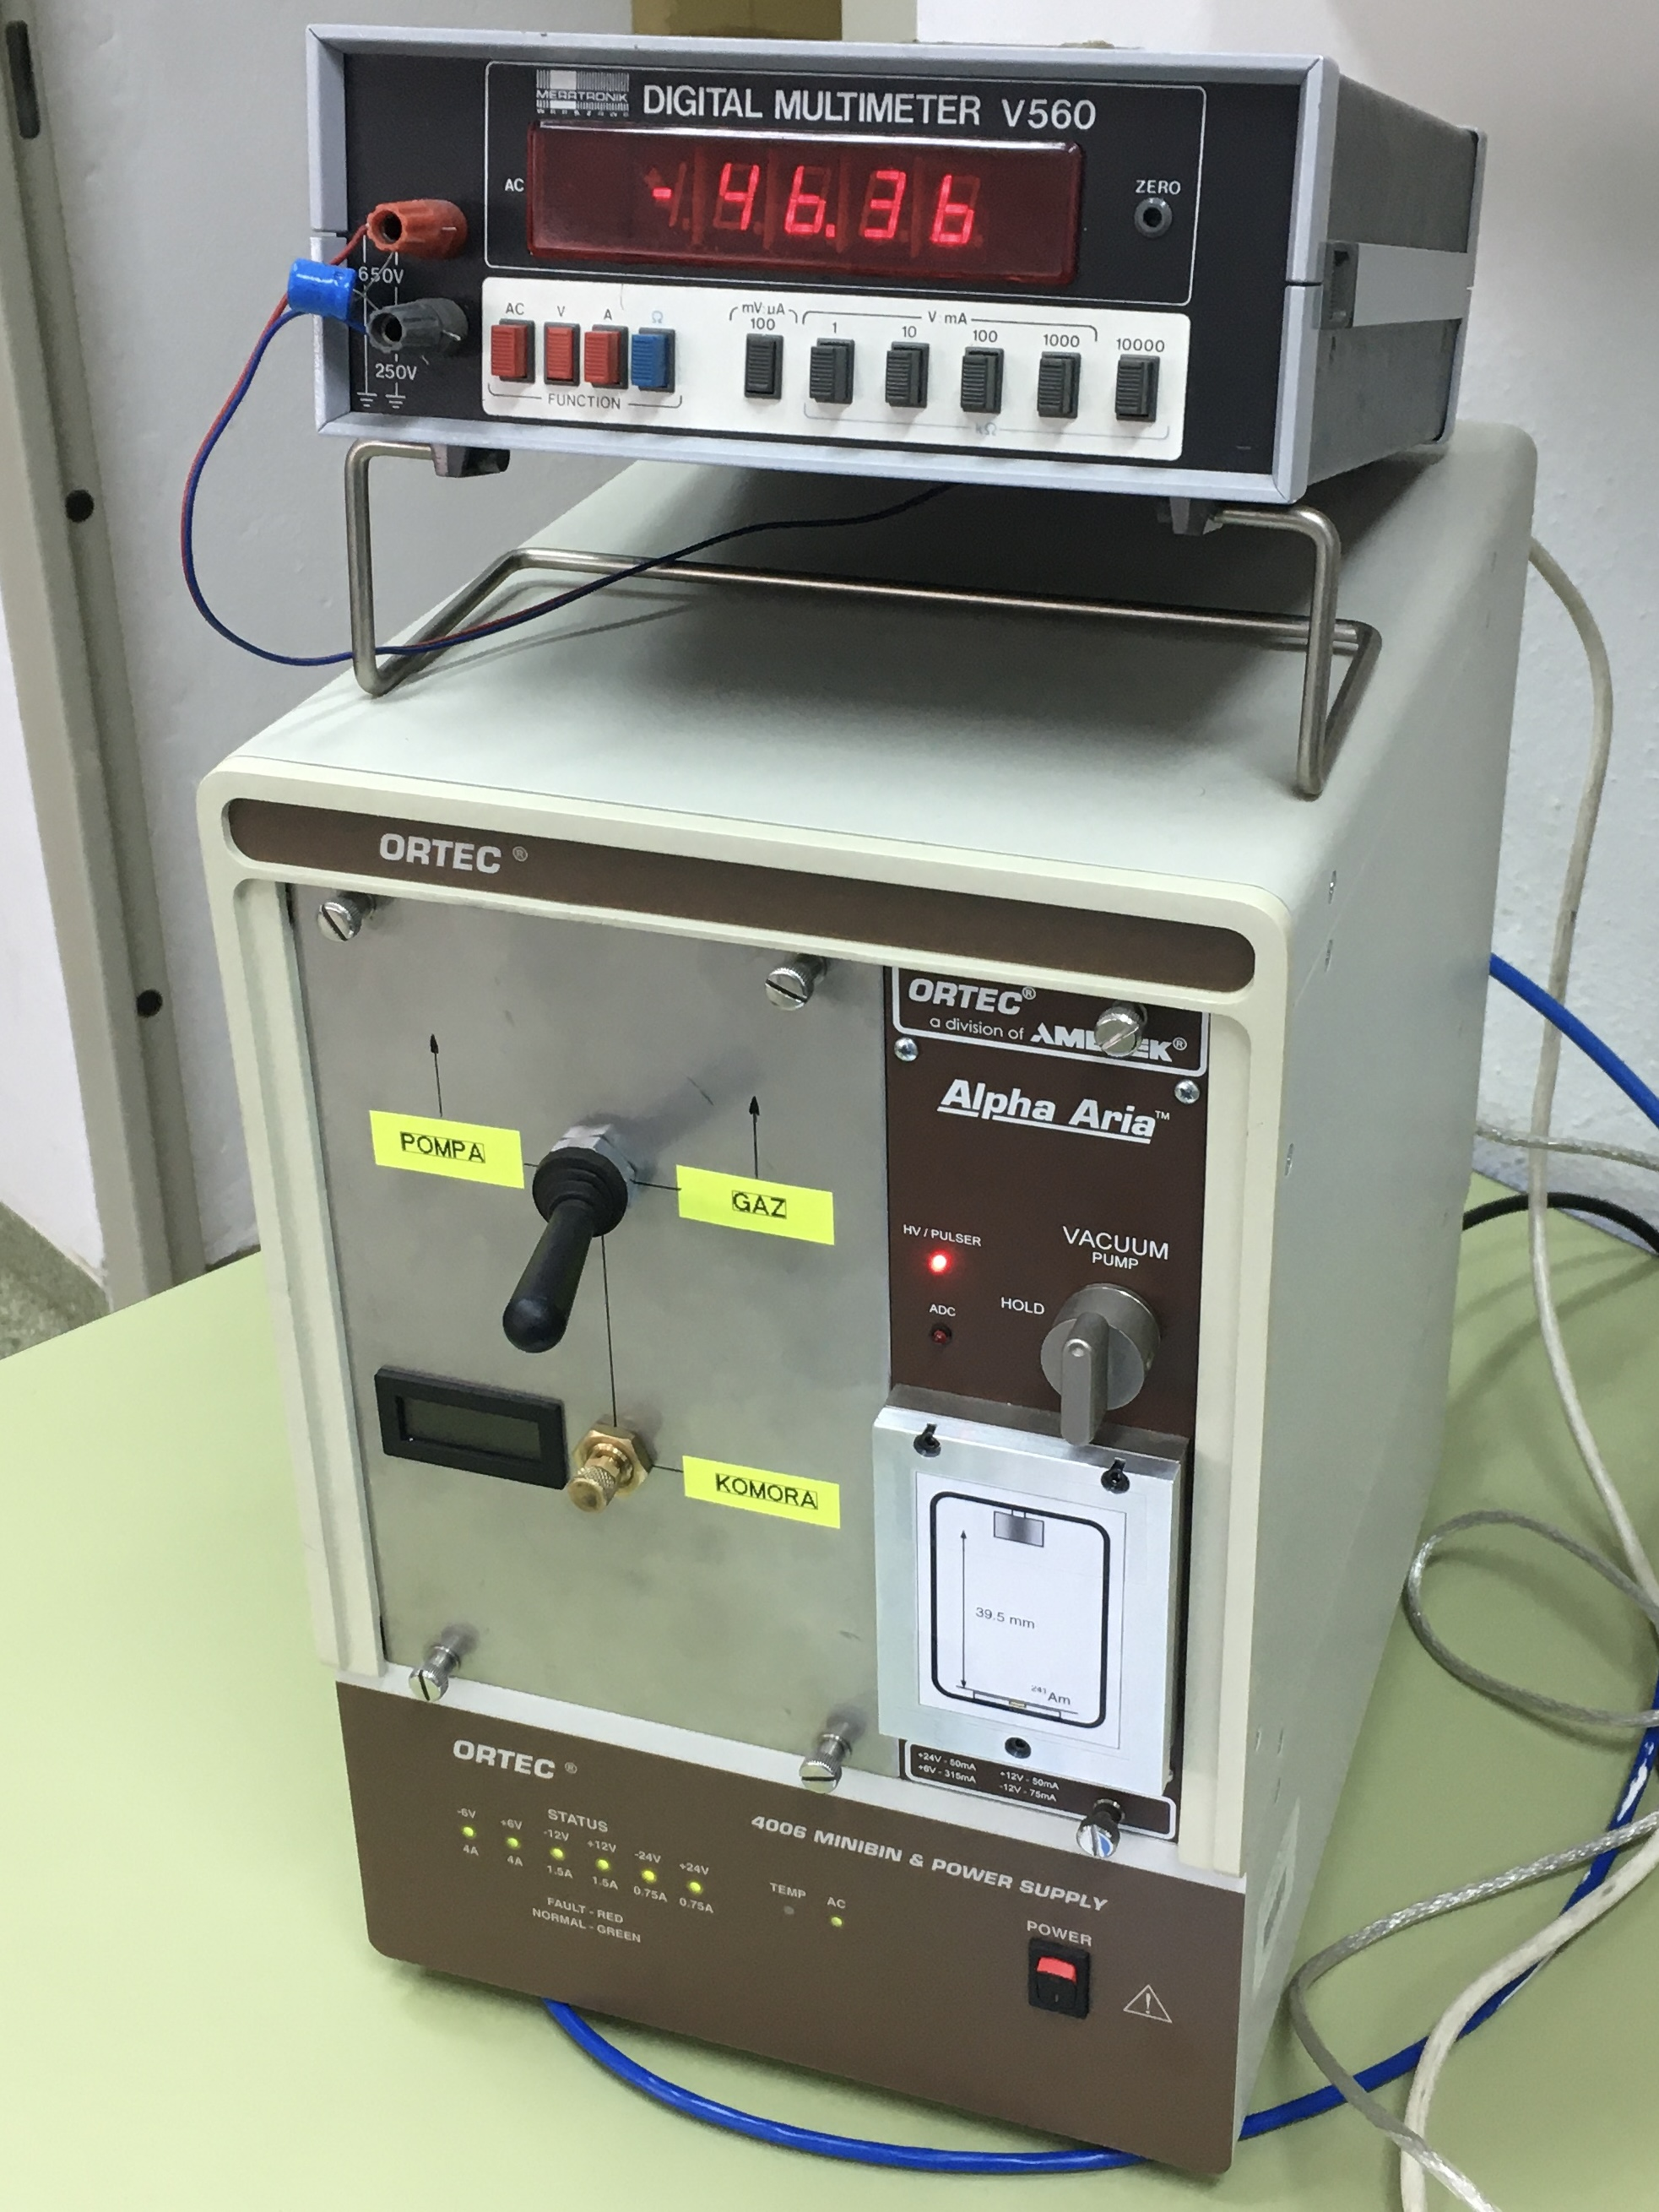
\includegraphics[keepaspectratio, width=0.8\linewidth]{zdj_uklad.JPG}
    \caption{Zdjęcie przedstawiające układ doświadczalny \cite{pracownia}}
    \label{fig:uklad}
\end{figure}

\section{Analiza i omówienie wyników}

W toku doświadczenia dokonano kilkunastu pomiarów dla różnych wartości ciśnienia w komorze, co jest widoczne na Rys. \ref{fig:wyniki_raw}. Każdy z pomiarów miał charakter widma energetycznego, zaś ciśnienie mierzone było poprzez wartość napięcia na woltomierzu podłączonym do barometru. Zmierzono wartości napięcia dla ciśnienia maksymalnego i minimalnego, a następnie dopasowano do tych pomiarów funkcję liniową, która służyła do przeliczania napięć na ciśnienia w barach, a te dalej na grubości warstwy absorbenta. Zliczenia w kanałach były za to przeliczane na energię cząstek zgodnie z procedurą opisaną wcześniej. Dane użyte do kalibracji energii widoczne są na Rys. \ref{fig:kal_energie}. Surowe dane z Rys. \ref{fig:wyniki_raw} zostały następnie przetłumaczone na wartości, które nas docelowo interesują: energię i grubość absorbenta w cm. Zostało to przedstawione na Rys. \ref{fig:dane_przeliczone}.

\begin{figure}[h!]
    \centering
    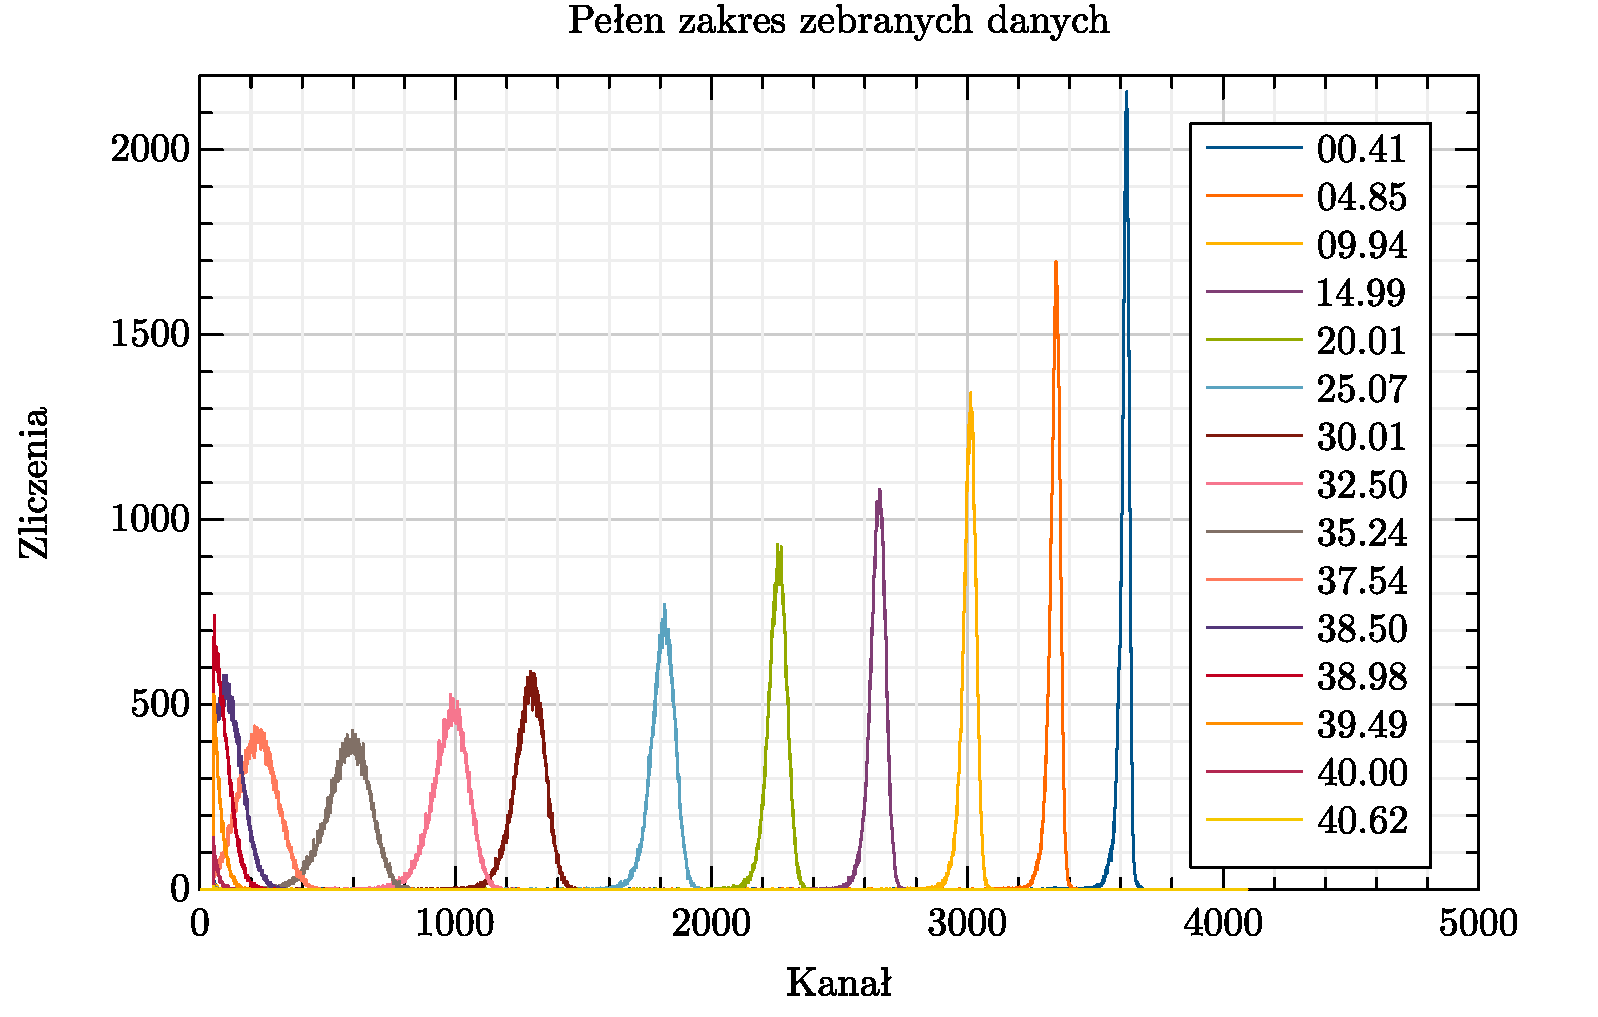
\includegraphics[keepaspectratio, width=0.8\linewidth]{peaks.pdf}
    \caption{Wykres przedstawiający wszystkie zarejestrowane widma wraz z napięciami - ciśnieniami dla których zostały zarejestrowane.}
    \label{fig:wyniki_raw}
\end{figure}

\begin{figure}[h!]
    \centering
    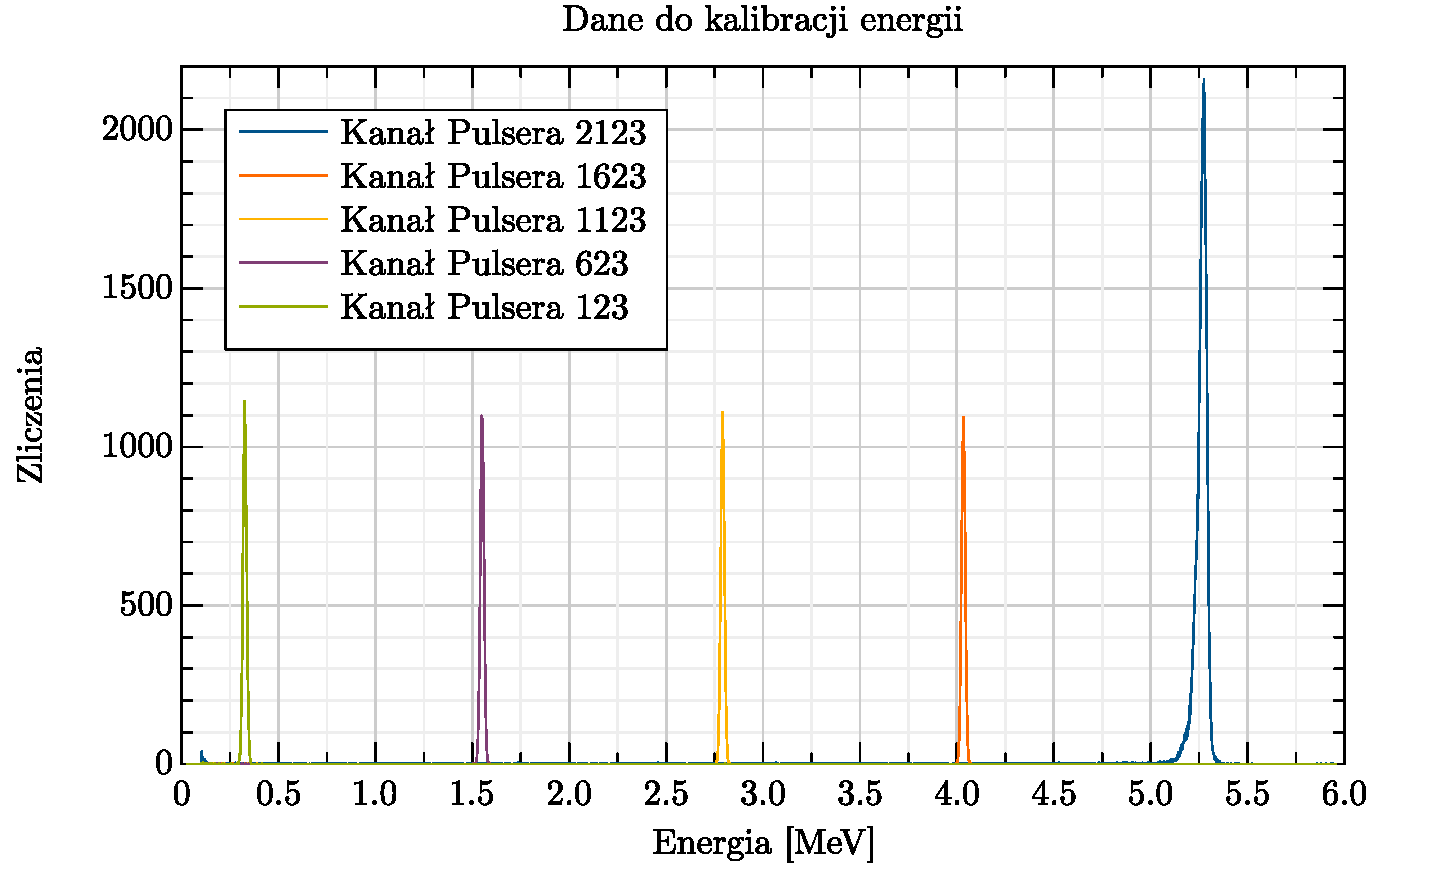
\includegraphics[keepaspectratio, width=0.8\linewidth]{peaks_kalibracja_energy.pdf}
    \caption{Wykres przedstawiający widma zarejestrowane do kalibracji korelacji numer kanału - energia}
    \label{fig:kal_energie}
\end{figure}

\begin{figure}[h!]
    \centering
    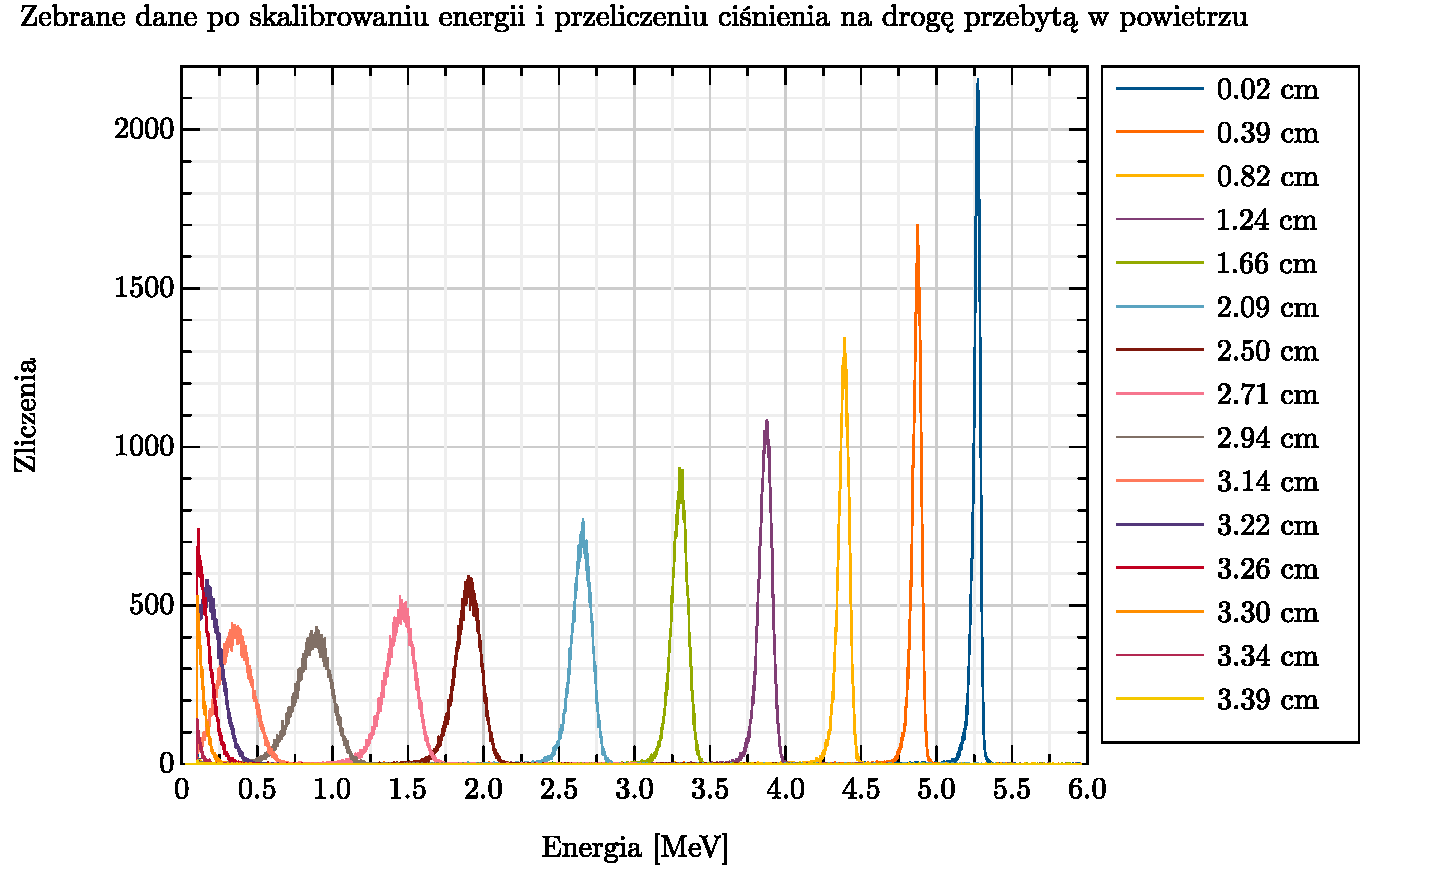
\includegraphics[keepaspectratio, width=0.8\linewidth]{peaks_energy.pdf}
    \caption{Wykres przedstawiający wszystkie zarejestrowane widma docelowych jednostkach.}
    \label{fig:dane_przeliczone}
\end{figure}

Idąc za wskazaniami \cite{publikacja} do danych widocznych na  Rys. \ref{fig:dane_przeliczone} dopasowywano rozkład Gaussa. Następnie wartości całkowitych liczb zliczeń w funkcji grubości absorbenta nam dają krzywą absorpcji, z której jesteśmy w stanie odczytać średni zasięg jako $\bar{R} = 3.253 \pm 0.002$\,cm i rozrzut zasięgu jako $\sigma_r = (8.649 \pm 0.004)\cdot 10^{-2}$\,cm, co jest wartościami zgodnymi z oczekiwaniami co do rzędu wielkości opartymi o wyniki zaprezentowane w publikacji \cite{publikacja}. Wykres przedstawiający krzywą absorpcji i wynikającą z niej pochodną - krzywą liczbowo-zasięgową widoczny jest na Rys. \ref{fig:absorpcja}.

\begin{figure}[h!]
    \centering
    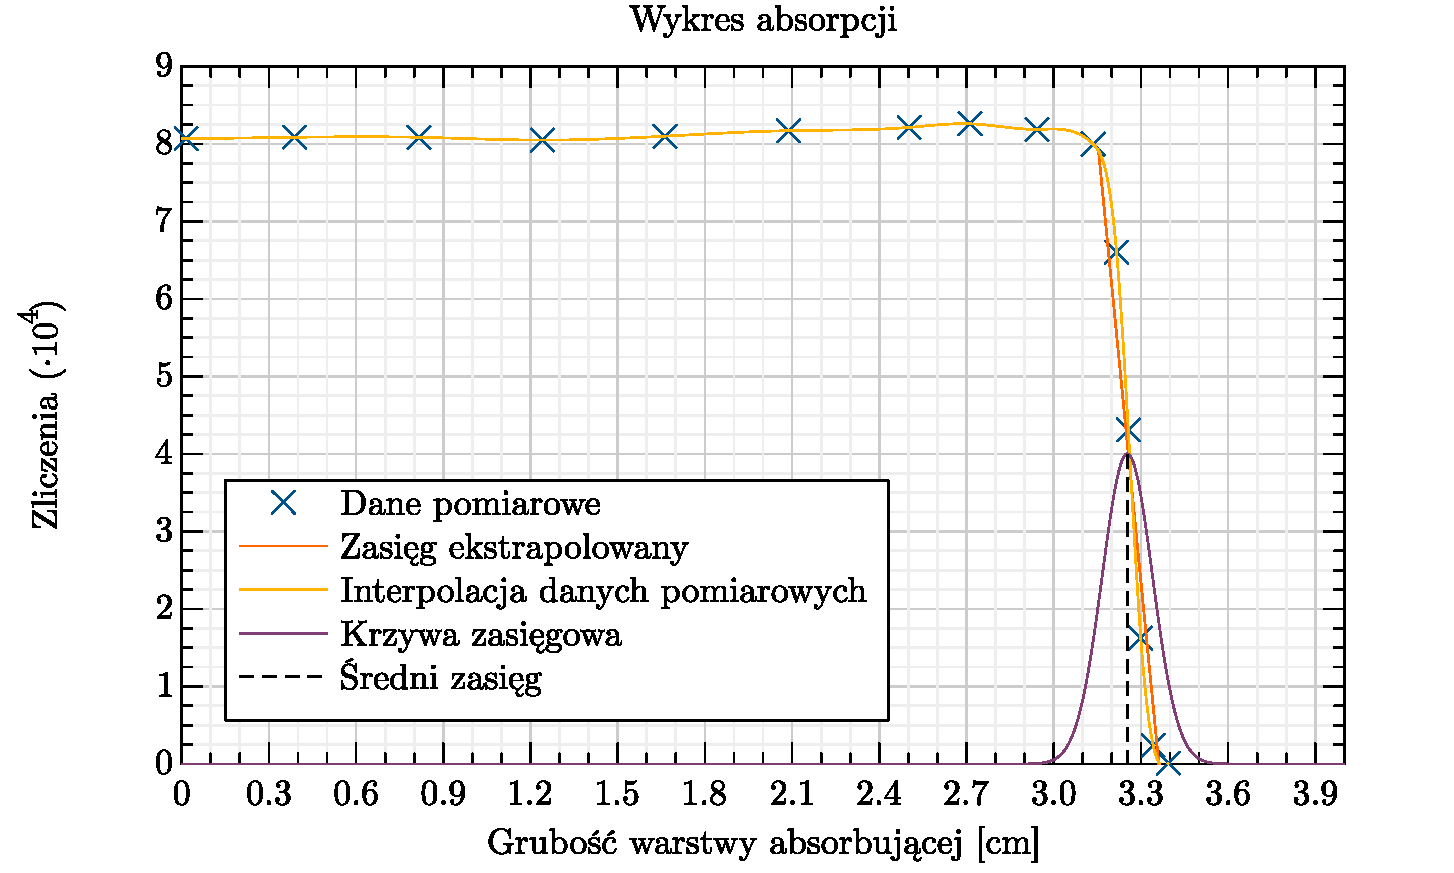
\includegraphics[keepaspectratio, width=0.8\linewidth]{absorpcja.pdf}
    \caption{Wykres przedstawiający krzywą absoropcji wraz z zaznaczonym średnim zasięgiem $\bar{R}$ i krzywą zmiany liczby zliczeń w postaci funkcji Gaussowskiej o wartości oczekiwanej $\bar{R}$ i wariancji $\sigma_r$.}
    \label{fig:absorpcja}
\end{figure}

\newpage

Kolejną szukaną charakterystyką była energia cząstki w zależności od grubości absorbenta. Wykres ten uzyskano poprzez naniesienie wartości oczekiwanych widocznych na Rys. \ref{fig:dane_przeliczone} na odpowiadające im grubości absorbentów. Uzyskanie tych danych jest niezbędnym krokiem do wyznaczenia zdolności hamującej $-\dd{E}/\dd{x}$ w funkcji grubości absorbenta, ponieważ dla naszych dyskretnych danych pomiarowych wartość tych strat energii była wyliczana jako $-\dd{E}/\dd{x} = - \Delta E / \Delta x$ gdzie pod $\Delta E$ rozumiemy różnicę energii dla dwóch kolejnych punktów pomiarowych, czy odpowiednio $\Delta x$ różnicę grubości. Dane te są widoczne na Rys. \ref{fig:stopping_power}. Widać jednoznacznie, że dane pomiarowe odpowiadające zdolności hamującej układają się w kształt przewidywany teoretycznie, tj. rosną do pewnego maksimum po to, a następnie gwałtownie spaść.

\begin{figure}[h!]
    \centering
    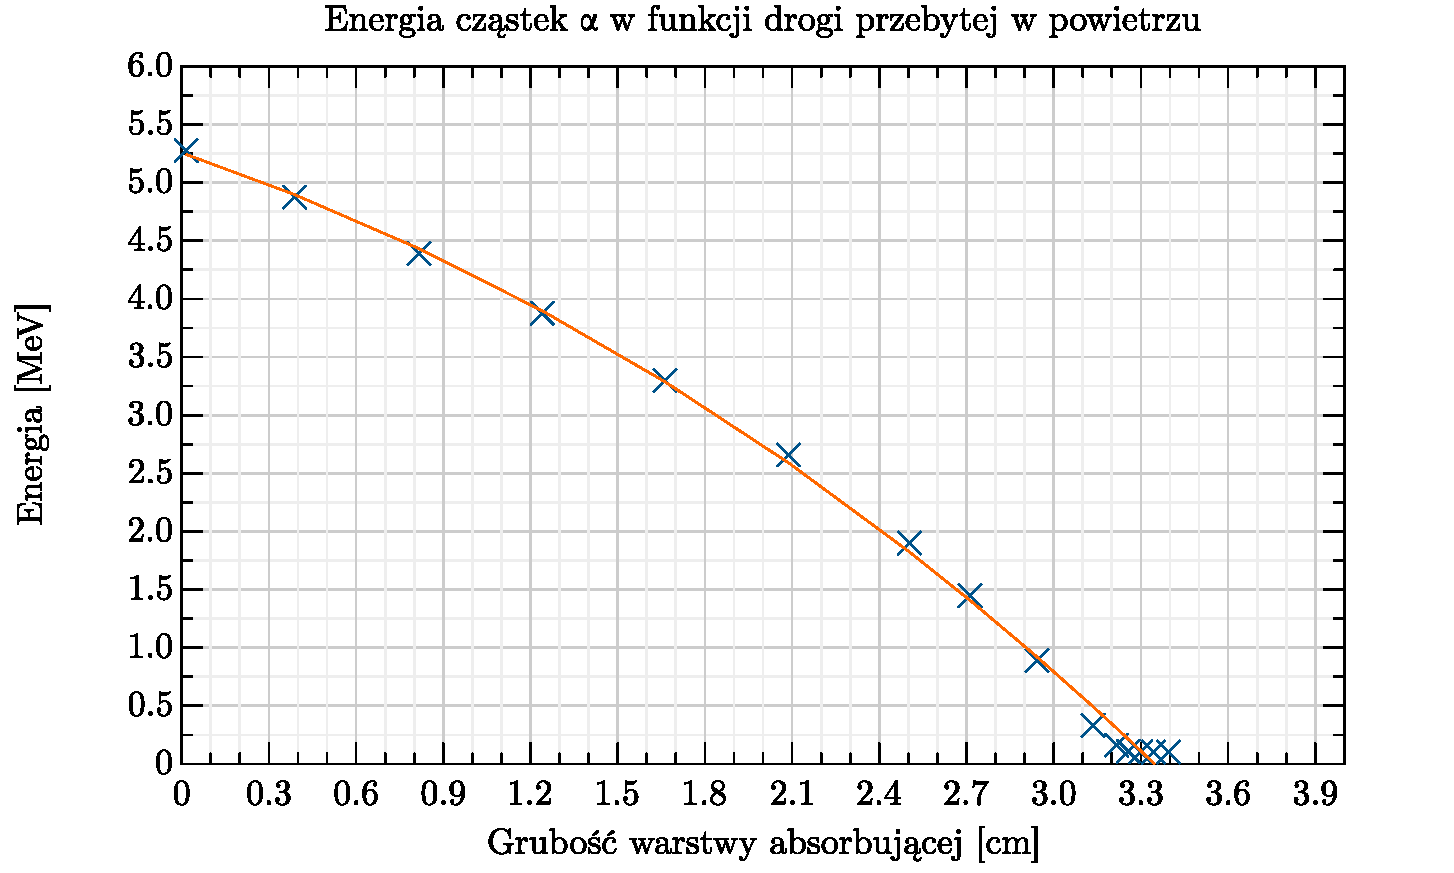
\includegraphics[keepaspectratio, width=0.8\linewidth]{energia_vs_absorber.pdf}
    \caption{Wykres przedstawiający energię cząstek $\alpha$ w funkcji grubości absorbenta.}
    \label{fig:energia_absorber}
\end{figure}

\begin{figure}[h!]
    \centering
    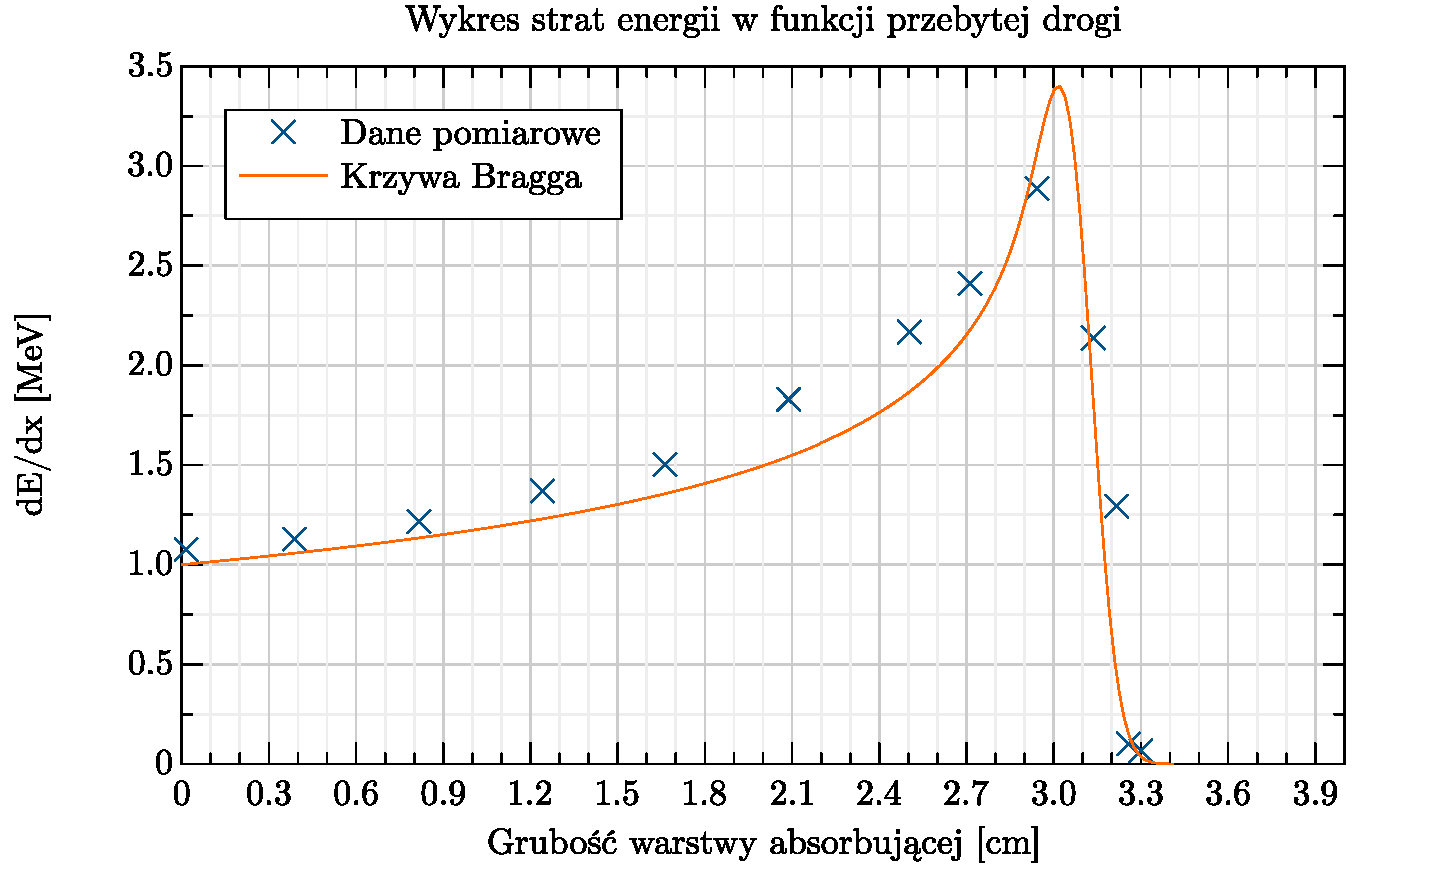
\includegraphics[keepaspectratio, width=0.8\linewidth]{bardziejkrzywaBragga.pdf}
    \caption{Wykres przedstawiający siłę hamującą w funkcji grubości absorbenta.}
    \label{fig:stopping_power}
\end{figure}

\FloatBarrier
\section{Podsumowanie}

W warunkach laboratorium w zasięgu studenta można było wyznaczyć ważne charakterystyki dla ciężkiej cząstki naładowanej w powietrzu, jaką jest cząstka $\alpha$. Przeprowadzono serię pomiarów, które następnie wykalibrowano, dopasowano do nich funkcje i w efekcie uzyskano pożądane zależności. Udało się wyznaczyć krzywą absorpcji cząstek $\alpha$ w powietrzu, zależność energii cząstki od grubości absorbenta, oraz zdolność hamującą w funkcji grubości absorbenta. Wyznaczono również średni zasięg i rozrzut cząstek $\alpha$ w powietrzu jako odpowiednio $\bar{R} = 3.253 \pm 0.002$\,cm i $\sigma_r = (8.649 \pm 0.004)\cdot 10^{-2}$\,cm.
  
\begin{thebibliography}{}
    \bibitem{strzalkowski}
    \textit{Wstęp do fizyki jądra atomowego} - A. Strzałkowski
    \bibitem{instrukcja}
    \href{https://www.fuw.edu.pl/IIPRACOWNIA/home/Opisy-cwiczen/J14_2018.pdf}{Instrukcja do doświadczenia}
    \bibitem{pracownia}\href{https://www.fuw.edu.pl/IIPRACOWNIA/home/}{Strona Pracowni dla Zaawansowanych}
    \bibitem{publikacja}
    \href{https://www.fuw.edu.pl/IIPRACOWNIA/home/Opisy-cwiczen/J14_2015.09.16_publikacja.pdf}{P. Ouseph, A. Mostovych Am. J Phys., Vol. \bf{46}, No.\bf{7} (1978)}, dostęp 05.07.2022
    
    
    
\end{thebibliography}
\end{document}